         \chapter{Vectors and scalars}
    \setcounter{figure}{1}
    \setcounter{subfigure}{1}
    \label{59e414b70efc194a27a122db47d06ce6}
         \section{ Introduction and key concepts}
    \nopagebreak
            \label{m38812} $ \hspace{-5pt}\begin{array}{cccccccccccc}   
\includegraphics[width=0.75cm]{col11305.imgs/summary_fullmarks.png} &   \end{array} $ \hspace{2 pt}\raisebox{-5 pt}{} {(section shortcode: P10091 )} \par 
    \label{m38812*cid2}
            \subsection{ Introduction}
            \nopagebreak
      \label{m38812*id186361}This chapter focuses on vectors. We will learn what is a vector and how it differs from everyday numbers. We will also learn how to add, subtract and multiply them and where they appear in Physics.\par 
      \label{m38812*id186366}Are vectors Physics? No, vectors themselves are not Physics. Physics is just a description of the world around us. To describe something we need to use a language. The most common language used to describe Physics is Mathematics. Vectors form a very important part of the mathematical description of Physics, so much so that it is
absolutely essential to master the use of vectors.\par 
    \label{m38812*cid3}
            \subsection{ Scalars and Vectors}
            \nopagebreak
      \label{m38812*id186720}In Mathematics, you learned that a number is something that represents a quantity. For example if you have 5 books, 6 apples and 1 bicycle, the 5, 6, and 1 represent how many of each item you have.\par 
      \label{m38812*id186725}These kinds of numbers are known as \textsl{scalars}.\par 
\label{m38812*fhsst!!!underscore!!!id78}\begin{definition}
	  \begin{tabular*}{15 cm}{m{15 mm}m{}}
	\hspace*{-50pt}  
\includegraphics[width=0.5in]{col11305.imgs/psflag2.png}   & \Definition{   \label{id2510220}\textbf{ Scalar }} { \label{m38812*meaningfhsst!!!underscore!!!id78}
      \label{m38812*id186740}A scalar is a quantity that has only magnitude (size). \par 
       } 
      \end{tabular*}
      \end{definition}
      \label{m38812*id186750}An extension to a scalar is a vector, which is a scalar with a direction. For example, if you travel 1 km down Main Road to school, the quantity \textbf{1 km down Main Road} is a vector. The ``\textbf{1 km}'' is the quantity (or scalar) and the ``\textbf{down Main Road}'' gives a direction.\par 
      \label{m38812*id186771}In Physics we use the word \textsl{magnitude} to refer to the scalar part of the vector.\par 
\label{m38812*fhsst!!!underscore!!!id83}\begin{definition}
	  \begin{tabular*}{15 cm}{m{15 mm}m{}}
	\hspace*{-50pt}  
\includegraphics[width=0.5in]{col11305.imgs/psflag2.png}   & \Definition{   \label{id2510284}\textbf{ Vectors }} { \label{m38812*meaningfhsst!!!underscore!!!id83}
      \label{m38812*id186786}A vector is a quantity that has both magnitude and direction. \par 
       } 
      \end{tabular*}
      \end{definition}
      \label{m38812*id186797}A vector should tell you \textbf{how much} and \textbf{which way}.\par 
      \label{m38812*id186810}For example, a man is driving his car east along a freeway at $100\phantom{\rule{2pt}{0ex}}\mathrm{km}\ensuremath{\cdot}\mathrm{h}{}^{-1}$. What we have given here is a vector -- the velocity. The car is moving at $100\phantom{\rule{2pt}{0ex}}\mathrm{km}\ensuremath{\cdot}\mathrm{h}{}^{-1}$ (this is the magnitude) and we know where it is going -- east (this is the direction). Thus, we know the speed and direction of the car. These two quantities, a magnitude and a direction, form a vector we call velocity.\par 
    \label{m38812*cid4}
            \subsection{ Notation}
            \nopagebreak
      \label{m38812*id186874}Vectors are different to scalars and therefore have their own notation.\par 
      \label{m38812*uid1}
            \subsubsection{ Mathematical Representation}
            \nopagebreak
        \label{m38812*id186887}There are many ways of writing the symbol for a vector. Vectors are denoted by symbols with an arrow pointing to the right above it. For example, $\stackrel{\to }{a}$, $\stackrel{\to }{v}$ and $\stackrel{\to }{F}$ represent the vectors acceleration, velocity and force, meaning they have both a magnitude and a direction.\par 
        \label{m38812*id186935}Sometimes just the magnitude of a vector is needed. In this case, the arrow is omitted. In other words, $F$ denotes the magnitude of the vector $\stackrel{\to }{F}$. \par 
      \label{m38812*uid2}
            \subsubsection{ Graphical Representation}
            \nopagebreak
        \label{m38812*id186285}Vectors are drawn as arrows. An arrow has both a magnitude (how long it is) and a direction (the direction in which it points). The starting point of a vector is known as the \textsl{tail} and the end point is known as the \textsl{head}.\par 
    \setcounter{subfigure}{0}
	\begin{figure}[H] % horizontal\label{m38812*uid3}
    \begin{center}
    \rule[.1in]{\figurerulewidth}{.005in} \\
        \label{m38812*uid3!!!underscore!!!media}\label{m38812*uid3!!!underscore!!!printimage}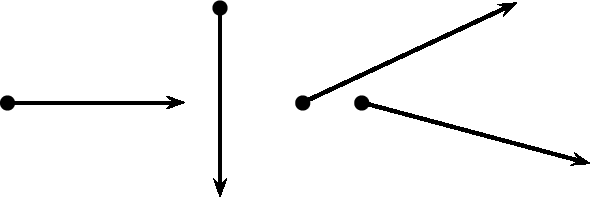
\includegraphics[width=5cm]{col11305.imgs/m38812_PG11C1_001.png} % m38812;PG11C1\_001.png;;;6.0;8.5;
      \vspace{2pt}
    \vspace{\rubberspace}\par \begin{cnxcaption}
	  \small \textbf{Figure 19.1: }Examples of vectors
	\end{cnxcaption}
    \vspace{.1in}
    \rule[.1in]{\figurerulewidth}{.005in} \\
    \end{center}
 \end{figure}       
    \setcounter{subfigure}{0}
	\begin{figure}[H] % horizontal\label{m38812*uid4}
    \begin{center}
    \rule[.1in]{\figurerulewidth}{.005in} \\
        \label{m38812*uid4!!!underscore!!!media}\label{m38812*uid4!!!underscore!!!printimage}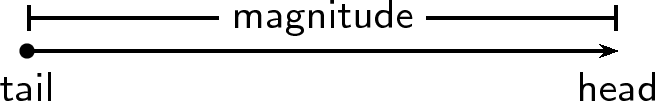
\includegraphics[width=6cm]{col11305.imgs/m38812_PG11C1_002.png} % m38812;PG11C1\_002.png;;;6.0;8.5;
      \vspace{2pt}
    \vspace{\rubberspace}\par \begin{cnxcaption}
	  \small \textbf{Figure 19.2: }Parts of a vector
	\end{cnxcaption}
    \vspace{.1in}
    \rule[.1in]{\figurerulewidth}{.005in} \\
    \end{center}
 \end{figure}       
    \label{m38812*cid5}
            \subsection{ Directions}
            \nopagebreak
      \label{m38812*id187219}There are many acceptable methods of writing vectors. As long as the vector has a magnitude and a direction, it is most likely acceptable. These different methods come from the different methods of expressing a direction for a vector.\par 
      \label{m38812*uid5}
            \subsubsection{ Relative Directions}
            \nopagebreak
        \label{m38812*id187233}The simplest method of expressing direction is with relative directions: to the left, to the right, forward, backward, up and down.\par 
      \label{m38812*uid6}
            \subsubsection{ Compass Directions}
            \nopagebreak
        \label{m38812*id187246}Another common method of expressing directions is to use the points of a compass: North, South, East, and West.
If a vector does not point exactly in one of the compass directions, then we use an angle. For example, we can have a vector pointing $40{}^{\circ }$ North of West. Start with the vector pointing along the West direction:
Then rotate the vector towards the north until there is a $40{}^{\circ }$ angle between the vector and the West.
The direction of this vector can also be described as: W $40{}^{\circ }$ N (West $40{}^{\circ }$ North); or N $50{}^{\circ }$ W (North $50{}^{\circ }$ West)
    \setcounter{subfigure}{0}
	\begin{figure}[H] % horizontal\label{m38812*id187349}
    \begin{center}
    \label{m38812*id187349!!!underscore!!!media}\label{m38812*id187349!!!underscore!!!printimage}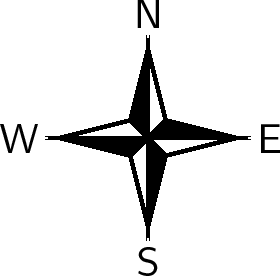
\includegraphics[width=2cm]{col11305.imgs/m38812_PG11C1_003.png} % m38812;PG11C1\_003.png;;;6.0;8.5;
      \vspace{2pt}
    \vspace{.1in}
    \end{center}
 \end{figure}       
    \setcounter{subfigure}{0}
	\begin{figure}[H] % horizontal\label{m38812*id187358}
    \begin{center}
    \label{m38812*id187358!!!underscore!!!media}\label{m38812*id187358!!!underscore!!!printimage}
\includegraphics[width=3cm]{col11305.imgs/m38812_PG11C1_004.png} % m38812;PG11C1\_004.png;;;6.0;8.5;
      \vspace{2pt}
    \vspace{.1in}
    \end{center}
 \end{figure}       
    \setcounter{subfigure}{0}
	\begin{figure}[H] % horizontal\label{m38812*id187367}
    \begin{center}
    \label{m38812*id187367!!!underscore!!!media}\label{m38812*id187367!!!underscore!!!printimage}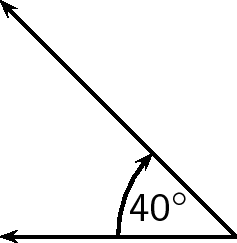
\includegraphics[width=3cm]{col11305.imgs/m38812_PG11C1_005.png} % m38812;PG11C1\_005.png;;;6.0;8.5;
      \vspace{2pt}
    \vspace{.1in}
    \end{center}
 \end{figure}       \par 
      \label{m38812*uid7}
            \subsubsection{ Bearing}
            \nopagebreak
        \label{m38812*id187384}The final method of expressing direction is to use a \textsl{bearing}. A bearing is a direction relative to a fixed point.\par 
        \label{m38812*id187393}Given just an angle, the convention is to define the angle with respect to the North. So, a vector with a direction of $110{}^{\circ }$ has been rotated clockwise $110{}^{\circ }$ relative to the North. A bearing is always written as a three digit number, for example $275{}^{\circ }$ or $080{}^{\circ }$ (for $80{}^{\circ }$).\par 
        \label{m38812*id187459}
    \setcounter{subfigure}{0}
	\begin{figure}[H] % horizontal\label{m38812*id187462}
    \begin{center}
    \label{m38812*id187462!!!underscore!!!media}\label{m38812*id187462!!!underscore!!!printimage}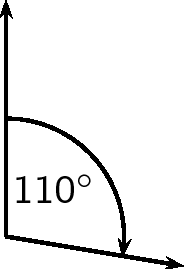
\includegraphics[width=3cm]{col11305.imgs/m38812_PG11C1_006.png} % m38812;PG11C1\_006.png;;;6.0;8.5;
      \vspace{2pt}
    \vspace{.1in}
    \end{center}
 \end{figure}       
        \par 
\label{m38812*secfhsst!!!underscore!!!id146}
            \subsubsection{  Scalars and Vectors }
            \nopagebreak
        \label{m38812*id187475}\begin{enumerate}[noitemsep, label=\textbf{\arabic*}. ] 
            \label{m38812*uid8}\item Classify the following quantities as scalars or vectors:
\label{m38812*id187490}\begin{enumerate}[noitemsep, label=\textbf{\alph*}. ] 
            \label{m38812*uid9}\item 12 km
\label{m38812*uid10}\item 1 m south
\label{m38812*uid11}\item $2\phantom{\rule{2pt}{0ex}}\mathrm{m}\ensuremath{\cdot}{\mathrm{s}}^{-1}$, $45{}^{\circ }$\label{m38812*uid12}\item $075{}^{\circ }$, 2 cm
\label{m38812*uid13}\item $100\phantom{\rule{2pt}{0ex}}\mathrm{k}\ensuremath{\cdot}{\mathrm{h}}^{-1}$, $0{}^{\circ }$\end{enumerate}
                \label{m38812*uid14}\item Use two different notations to write down the direction of the vector in each of the following diagrams:
\label{m38812*id187643}\begin{enumerate}[noitemsep, label=\textbf{\alph*}. ] 
            \label{m38812*uid15}\item 
    \setcounter{subfigure}{0}
	\begin{figure}[H] % horizontal\label{m38812*id187654}
    \begin{center}
    \label{m38812*id187654!!!underscore!!!media}\label{m38812*id187654!!!underscore!!!printimage}
\includegraphics[height=2cm]{col11305.imgs/m38812_PG11C1_007.png} % m38812;PG11C1\_007.png;;;6.0;8.5;
      \vspace{2pt}
    \vspace{.1in}
    \end{center}
 \end{figure}       \label{m38812*uid16}\item 
    \setcounter{subfigure}{0}
	\begin{figure}[H] % horizontal\label{m38812*id187668}
    \begin{center}
    \label{m38812*id187668!!!underscore!!!media}\label{m38812*id187668!!!underscore!!!printimage}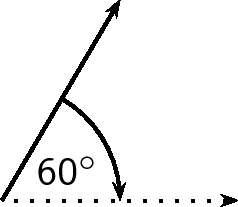
\includegraphics[width=3cm]{col11305.imgs/m38812_PG11C1_008.png} % m38812;PG11C1\_008.png;;;6.0;8.5;
      \vspace{2pt}
    \vspace{.1in}
    \end{center}
 \end{figure}       \label{m38812*uid17}\item 
    \setcounter{subfigure}{0}
	\begin{figure}[H] % horizontal\label{m38812*id187683}
    \begin{center}
    \label{m38812*id187683!!!underscore!!!media}\label{m38812*id187683!!!underscore!!!printimage}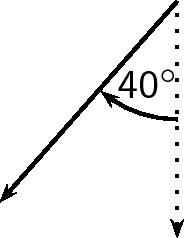
\includegraphics[width=3cm]{col11305.imgs/m38812_PG11C1_009.png} % m38812;PG11C1\_009.png;;;6.0;8.5;
      \vspace{2pt}
    \vspace{.1in}
    \end{center}
 \end{figure}       \end{enumerate}
                \end{enumerate}
    \label{m38812*cid6}
\par \raisebox{-5 pt}{
\includegraphics[width=0.5cm]{col11305.imgs/summary_www.png}} Find the answers with the shortcodes:
 \par \begin{tabular}[h]{cccccc}
 (1.) l4s  &  (2.) l4H  & \end{tabular}
            \subsection{ Drawing Vectors}
            \nopagebreak
      \label{m38812*id187709}In order to draw a vector accurately we must specify a scale and
include a reference direction in the diagram. A scale allows us to
translate the length of the arrow into the vector's magnitude. For
instance if one chose a scale of 1 cm = 2 N (1 cm represents 2 N), a
force of 20 N towards the East would be represented as an arrow 10 cm
long. A reference direction may be a line representing a horizontal surface or the points of a compass.\par 
      \label{m38812*id187716}
    \setcounter{subfigure}{0}
	\begin{figure}[H] % horizontal\label{m38812*id187719}
    \begin{center}
    \label{m38812*id187719!!!underscore!!!media}\label{m38812*id187719!!!underscore!!!printimage}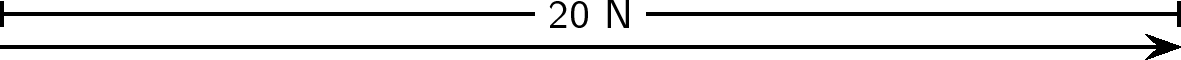
\includegraphics[width=5cm]{col11305.imgs/m38812_PG11C1_010.png} % m38812;PG11C1\_010.png;;;6.0;8.5;
      \vspace{2pt}
    \vspace{.1in}
    \end{center}
 \end{figure}       
      \par 
      \label{m38812*id187725}
        \textbf{Method: Drawing Vectors}
        \label{m38812*id187736}\begin{enumerate}[noitemsep, label=\textbf{\arabic*}. ] 
            \label{m38812*uid18}\item Decide upon a scale and write it down.
\label{m38812*uid19}\item Determine the length of the arrow representing the vector, by using the scale.
\label{m38812*uid20}\item Draw the vector as an arrow. Make sure that you fill in the arrow head.
\label{m38812*uid21}\item Fill in the magnitude of the vector.
\end{enumerate}
      \par 
\par
            \label{m38812*secfhsst!!!underscore!!!id189}\vspace{.5cm} 
      \noindent
      \hspace*{-30pt}
\includegraphics[width=0.5in]{col11305.imgs/pspencil2.png}   \raisebox{25mm}{   
      \begin{mdframed}[linewidth=4, leftmargin=40, rightmargin=40]  
      \begin{exercise}
    \noindent\textbf{Exercise 19.1:  Drawing vectors }
      \label{m38812*probfhsst!!!underscore!!!id190}
      \label{m38812*id187800}Represent the following vector quantities:\par 
      \label{m38812*id187805}\begin{enumerate}[noitemsep, label=\textbf{\arabic*}. ] 
            \leftskip=20pt\rightskip=\leftskip\label{m38812*uid22}\item $6\phantom{\rule{2pt}{0ex}}\mathrm{m}\ensuremath{\cdot}{\mathrm{s}}^{-1}$ north
\label{m38812*uid23}\item 16 m east
\end{enumerate}
      \vspace{5pt}
      \label{m38812*solfhsst!!!underscore!!!id200}\noindent\textbf{Solution to Exercise } \label{m38812*listfhsst!!!underscore!!!id200}\begin{enumerate}[noitemsep, label=\textbf{Step} \textbf{\arabic*}. ] 
            \leftskip=20pt\rightskip=\leftskip\item  
      \label{m38812*id187874}\begin{enumerate}[noitemsep, label=\textbf{\alph*}. ] 
            \leftskip=20pt\rightskip=\leftskip\label{m38812*uid24}\item $1\phantom{\rule{2pt}{0ex}}\mathrm{cm}=2\phantom{\rule{2pt}{0ex}}\mathrm{m}\ensuremath{\cdot}{\mathrm{s}}^{-1}$\label{m38812*uid25}\item $1\phantom{\rule{2pt}{0ex}}\mathrm{cm}=4\phantom{\rule{2pt}{0ex}}\mathrm{m}$
\end{enumerate}
      \item  
      \label{m38812*id187925}\begin{enumerate}[noitemsep, label=\textbf{\alph*}. ] 
            \leftskip=20pt\rightskip=\leftskip\label{m38812*uid26}\item If $1\phantom{\rule{2pt}{0ex}}\mathrm{cm}=2\phantom{\rule{2pt}{0ex}}\mathrm{m}\ensuremath{\cdot}{\mathrm{s}}^{-1}$, then $6\phantom{\rule{2pt}{0ex}}\mathrm{m}\ensuremath{\cdot}{\mathrm{s}}^{-1}=3\phantom{\rule{2pt}{0ex}}\mathrm{cm}$
\label{m38812*uid27}\item If $1\phantom{\rule{2pt}{0ex}}\mathrm{cm}=4\phantom{\rule{2pt}{0ex}}\mathrm{m}$, then $16\phantom{\rule{2pt}{0ex}}\mathrm{m}=4\phantom{\rule{2pt}{0ex}}\mathrm{cm}$
\end{enumerate}
      \item  
      \label{m38812*id188000}\begin{enumerate}[noitemsep, label=\textbf{\alph*}. ] 
            \leftskip=20pt\rightskip=\leftskip\label{m38812*uid28}\item 
Scale used: $1\phantom{\rule{2pt}{0ex}}\mathrm{cm}=2\phantom{\rule{2pt}{0ex}}\mathrm{m}\ensuremath{\cdot}{\mathrm{s}}^{-1}$
Direction = North
    \setcounter{subfigure}{0}
	\begin{figure}[H] % horizontal\label{m38812*id188039}
    \begin{center}
    \label{m38812*id188039!!!underscore!!!media}\label{m38812*id188039!!!underscore!!!printimage}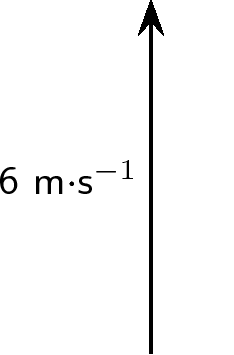
\includegraphics{col11305.imgs/m38812_PG11C1_011.png} % ;PG11C1\_011.png;;;6.0;8.5;
      \vspace{2pt}
    \vspace{.1in}
    \end{center}
 \end{figure}       \label{m38812*uid29}\item 
Scale used: $1\phantom{\rule{2pt}{0ex}}\mathrm{cm}=4\phantom{\rule{2pt}{0ex}}\mathrm{m}$
Direction = East
    \setcounter{subfigure}{0}
	\begin{figure}[H] % horizontal\label{m38812*id188060}
    \begin{center}
    \label{m38812*id188060!!!underscore!!!media}\label{m38812*id188060!!!underscore!!!printimage}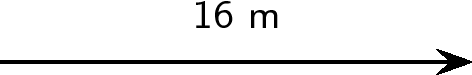
\includegraphics{col11305.imgs/m38812_PG11C1_012.png} % ;PG11C1\_012.png;;;6.0;8.5;
      \vspace{2pt}
    \vspace{.1in}
    \end{center}
 \end{figure}       \end{enumerate}
      \end{enumerate}
    \end{exercise}
    \end{mdframed}
    }
    \noindent
\label{m38812*secfhsst!!!underscore!!!id228}
            \subsubsection{ Drawing Vectors }
            \nopagebreak
            \label{m38812*id188088}Draw each of the following vectors to scale. Indicate the scale that you have used:
      \label{m38812*id188094}\begin{enumerate}[noitemsep, label=\textbf{\arabic*}. ] 
            \label{m38812*uid30}\item 12 km south
\label{m38812*uid31}\item 1,5 m N $45{}^{\circ }$ W
\label{m38812*uid32}\item $1\phantom{\rule{2pt}{0ex}}\mathrm{m}\ensuremath{\cdot}\mathrm{s}{}^{-1}$, $20{}^{\circ }$ East of North
\label{m38812*uid33}\item $50\phantom{\rule{2pt}{0ex}}\mathrm{km}\ensuremath{\cdot}\mathrm{h}{}^{-1}$, $085{}^{\circ }$\label{m38812*uid34}\item 5 mm, $225{}^{\circ }$\end{enumerate}
                \par 
  \label{m38812**end}
\par \raisebox{-5 pt}{
\includegraphics[width=0.5cm]{col11305.imgs/summary_www.png}} Find the answers with the shortcodes:
 \par \begin{tabular}[h]{cccccc}
 (1.) l46  & \end{tabular}
         \section{ Mathematical properties}
    \nopagebreak
            \label{m38813} $ \hspace{-5pt}\begin{array}{cccccccccccc}   \end{array} $ \hspace{2 pt}\raisebox{-5 pt}{
\includegraphics[width=0.5cm]{col11305.imgs/summary_www.png}} {(section shortcode: P10092 )} \par 
    \label{m38813*cid7}
            \subsection{ Mathematical Properties of Vectors}
            \nopagebreak
      \label{m38813*id188277}Vectors are mathematical objects and we need to understand the mathematical properties of vectors, like adding and subtracting.\par 
      \label{m38813*id188281}For all the examples in this section, we will use displacement as our vector quantity. Displacement was discussed in
Grade 10.\par 
      \label{m38813*id188286}Displacement is defined as the distance together with direction of the straight line joining a final point to an initial point.\par 
      \label{m38813*id188290}Remember that displacement is just one example of a vector. We could just as well have decided to use forces or velocities to illustrate the properties of vectors.\par 
      \label{m38813*uid35}
            \subsubsection{ Adding Vectors}
            \nopagebreak
        \label{m38813*id188304}When vectors are added, we need to add both a magnitude \textbf{and} a direction. For example, take 2 steps in the forward direction, stop and then take another 3 steps in the forward direction. The first 2 steps is a displacement vector and the second 3 steps is also a displacement vector. If we did not stop after the first 2 steps, we would have taken 5 steps in the forward direction in total. Therefore, if we add the displacement vectors for 2 steps and 3 steps, we should get a total of 5 steps in the forward direction. Graphically, this can be seen by first following the first vector two steps forward and then following the second one three steps forward (ie. in the same direction):\par 
        \label{m38813*id188318}
    \setcounter{subfigure}{0}
	\begin{figure}[H] % horizontal\label{m38813*id188322}
    \begin{center}
    \label{m38813*id188322!!!underscore!!!media}\label{m38813*id188322!!!underscore!!!printimage}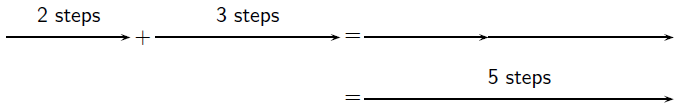
\includegraphics[width=300px]{col11305.imgs/m38813_PG11C1_013.png} % m38813;PG11C1\_013.png;;;6.0;8.5;
      \vspace{2pt}
    \vspace{.1in}
    \end{center}
 \end{figure}       
        \par 
        \label{m38813*id188328}We add the second vector at the end of the first vector, since this is where we now are after the first vector has acted. The vector from the tail of the
first vector (the starting point) to the head of the last (the end
point) is then the sum of the vectors. This is the \textsl{head-to-tail} method of vector addition.\par 
        \label{m38813*id188340}As you can convince yourself, the order in which you add vectors does
not matter. In the example above, if you decided to first go 3 steps
forward and then another 2 steps forward, the end result would still be 5
steps forward.\par 
        \label{m38813*id188345}The final answer when adding vectors is called the \textbf{resultant}. The resultant displacement in this case will be 5 steps forward.\par 
\label{m38813*fhsst!!!underscore!!!id269}\begin{definition}
	  \begin{tabular*}{15 cm}{m{15 mm}m{}}
	\hspace*{-50pt}  
\includegraphics[width=0.5in]{col11305.imgs/psflag2.png}   & \Definition{   \label{id2512331}\textbf{ Resultant of Vectors }} { \label{m38813*meaningfhsst!!!underscore!!!id269}
        \label{m38813*id188362}The resultant of a number of vectors is the single vector whose effect is the same as the individual vectors acting together. \par 
         } 
      \end{tabular*}
      \end{definition}
        \label{m38813*id188374}In other words, the individual vectors can be replaced by the
resultant -- the overall effect is the same. If vectors $\stackrel{\to }{a}$ and $\stackrel{\to }{b}$ have a resultant $\stackrel{\to }{R}$, this can be represented mathematically as,\par 
        \label{m38813*id188427}\nopagebreak\noindent{}
          
    \begin{equation}
    \begin{array}{ccc}\hfill \stackrel{\to }{R}& =& \stackrel{\to }{a}+\stackrel{\to }{b}.\hfill \end{array}\tag{19.1}
      \end{equation}
        \label{m38813*id188482}Let us consider some more examples of vector addition using displacements. The arrows tell you how far to move and in what
direction. Arrows to the right correspond to steps forward, while
arrows to the left correspond to steps backward. Look at all of the
examples below and check them.\par 
        \label{m38813*id186651}
    \setcounter{subfigure}{0}
	\begin{figure}[H] % horizontal\label{m38813*id186654}
    \begin{center}
    \label{m38813*id186654!!!underscore!!!media}\label{m38813*id186654!!!underscore!!!printimage}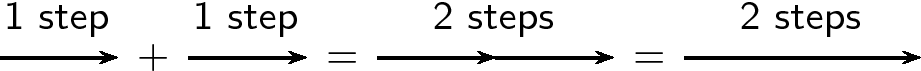
\includegraphics[width=300px]{col11305.imgs/m38813_PG11C1_014.png} % m38813;PG11C1\_014.png;;;6.0;8.5;
      \vspace{2pt}
    \vspace{.1in}
    \end{center}
 \end{figure}       
        \par 
        \label{m38813*id186661}This example says 1 step forward and then another step forward is the same as an arrow twice as long -- two steps forward.\par 
        \label{m38813*id186668}
    \setcounter{subfigure}{0}
	\begin{figure}[H] % horizontal\label{m38813*id186672}
    \begin{center}
    \label{m38813*id186672!!!underscore!!!media}\label{m38813*id186672!!!underscore!!!printimage}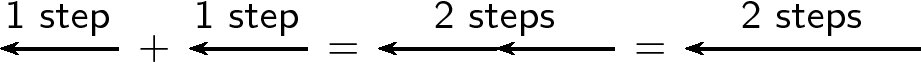
\includegraphics[width=300px]{col11305.imgs/m38813_PG11C1_015.png} % m38813;PG11C1\_015.png;;;6.0;8.5;
      \vspace{2pt}
    \vspace{.1in}
    \end{center}
 \end{figure}       
        \par 
        \label{m38813*id186678}This examples says 1 step backward and then another step backward is the same as an arrow twice as long -- two steps backward.\par 
        \label{m38813*id186684}It is sometimes possible that you end up back where you started. In this case the net result of what you have done is that you have gone nowhere
(your start and end points are at the same place). In this case, your resultant displacement is a vector with length zero units. We use the symbol $\stackrel{\to }{0}$ to denote such a vector:\par 
        \label{m38813*id186706}
    \setcounter{subfigure}{0}
	\begin{figure}[H] % horizontal\label{m38813*id186710}
    \begin{center}
    \label{m38813*id186710!!!underscore!!!media}\label{m38813*id186710!!!underscore!!!printimage}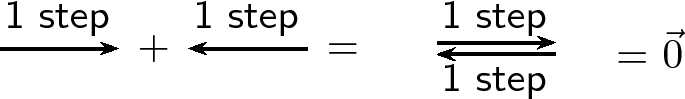
\includegraphics[width=6cm]{col11305.imgs/m38813_PG11C1_016.png} % m38813;PG11C1\_016.png;;;6.0;8.5;
      \vspace{2pt}
    \vspace{.1in}
    \end{center}
 \end{figure}       
        \par 
        \label{m38813*id186716}
    \setcounter{subfigure}{0}
	\begin{figure}[H] % horizontal\label{m38813*id188625}
    \begin{center}
    \label{m38813*id188625!!!underscore!!!media}\label{m38813*id188625!!!underscore!!!printimage}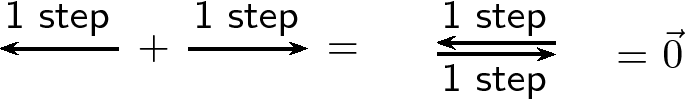
\includegraphics[width=6cm]{col11305.imgs/m38813_PG11C1_017.png} % m38813;PG11C1\_017.png;;;6.0;8.5;
      \vspace{2pt}
    \vspace{.1in}
    \end{center}
 \end{figure}       
        \par 
        \label{m38813*id188632}Check the following examples in the same way. Arrows up the page can be
seen as steps left and arrows down the page as steps right.\par 
        \label{m38813*id188636}Try a couple to convince yourself!\par \nopagebreak
    % \textbf{m38813*id188639}\par
          \begin{table}[H]
    % \begin{table}[H]
    % \\ 'id2994190' '1'
        \begin{center}
      \label{m38819*id197541}
    \noindent
    \tabletail{%
        \hline
        \multicolumn{3}{|p{\mytableboxwidth}|}{\raggedleft \small \sl continued on next page}\\
        \hline
      }
      \tablelasttail{}
      \begin{xtabular}[t]{|l|l|l|}\hline
         &
        P &
        Q% make-rowspan-placeholders
     \tabularnewline\cline{1-1}\cline{2-2}\cline{3-3}
      %--------------------------------------------------------------------
        A &
        100 N &
        0 N% make-rowspan-placeholders
     \tabularnewline\cline{1-1}\cline{2-2}\cline{3-3}
      %--------------------------------------------------------------------
        B &
        25 N &
        75 N% make-rowspan-placeholders
     \tabularnewline\cline{1-1}\cline{2-2}\cline{3-3}
      %--------------------------------------------------------------------
        C &
        50 N &
        50 N% make-rowspan-placeholders
     \tabularnewline\cline{1-1}\cline{2-2}\cline{3-3}
      %--------------------------------------------------------------------
        D &
        100 N &
        100 N% make-rowspan-placeholders
     \tabularnewline\cline{1-1}\cline{2-2}\cline{3-3}
      %--------------------------------------------------------------------
    \end{xtabular}
      \end{center}
    \begin{center}{\small\bfseries Table 19.10}\end{center}
    \begin{caption}{\small\bfseries Table 19.10}\end{caption}
\end{table}
    \par
          \label{m38819*uid92}\item A point is acted on by two forces in equilibrium. The forces
\label{m38819*id197705}\begin{enumerate}[noitemsep, label=\textbf{\alph*}. ] 
            \label{m38819*uid93}\item have equal magnitudes and directions.
\label{m38819*uid94}\item have equal magnitudes but opposite directions.
\label{m38819*uid95}\item act perpendicular to each other.
\label{m38819*uid96}\item act in the same direction.
\end{enumerate}
                \label{m38819*uid97}\item A point in equilibrium is acted on by three forces. Force ${F}_{1}$ has components 15 N due south and 13 N due west. What are the components of force ${F}_{2}$?
\label{m38819*id197809}\begin{enumerate}[noitemsep, label=\textbf{\alph*}. ] 
            \label{m38819*uid98}\item 13 N due north and 20 due west
\label{m38819*uid99}\item 13 N due north and 13 N due west
\label{m38819*uid100}\item 15 N due north and 7 N due west
\label{m38819*uid101}\item 15 N due north and 13 N due east
\end{enumerate}
    \setcounter{subfigure}{0}
	\begin{figure}[H] % horizontal\label{m38819*id197871}
    \begin{center}
    \label{m38819*id197871!!!underscore!!!media}\label{m38819*id197871!!!underscore!!!printimage}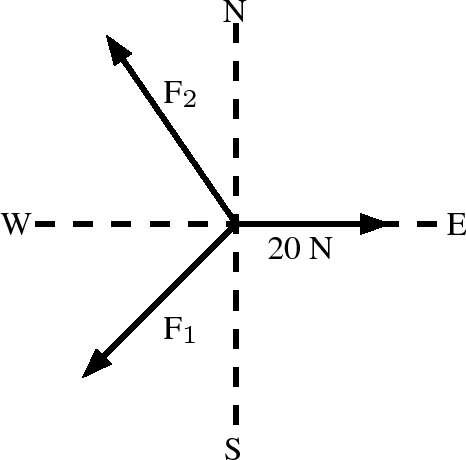
\includegraphics[width=3cm]{col11305.imgs/m38819_PG11C1_079.png} % m38819;PG11C1\_079.png;;;6.0;8.5;
      \vspace{2pt}
    \vspace{.1in}
    \end{center}
 \end{figure}               \label{m38819*uid102}\item Which of the following contains two vectors and a scalar?
\label{m38819*id197890}\begin{enumerate}[noitemsep, label=\textbf{\alph*}. ] 
            \label{m38819*uid103}\item distance, acceleration, speed
\label{m38819*uid104}\item displacement, velocity, acceleration
\label{m38819*uid105}\item distance, mass, speed
\label{m38819*uid106}\item displacement, speed, velocity
\end{enumerate}
                \label{m38819*uid107}\item Two vectors act on the same point. What should the angle between them be so that a maximum resultant is obtained?
\label{m38819*id197965}\begin{enumerate}[noitemsep, label=\textbf{\alph*}. ] 
            \label{m38819*uid108}\item $0{}^{\circ }$\label{m38819*uid109}\item $90{}^{\circ }$\label{m38819*uid110}\item $180{}^{\circ }$\label{m38819*uid111}\item cannot tell
\end{enumerate}
                \label{m38819*uid112}\item Two forces, 4~N and 11~N, act on a point. Which one of the following \uline{cannot} be the magnitude of a resultant?
\label{m38819*id198082}\begin{enumerate}[noitemsep, label=\textbf{\alph*}. ] 
            \label{m38819*uid113}\item 4 N
\label{m38819*uid114}\item 7 N
\label{m38819*uid115}\item 11 N
\label{m38819*uid116}\item 15 N
\end{enumerate}
        \newline
            \end{enumerate}
      \label{m38819*uid117}
\par \raisebox{-5 pt}{
\includegraphics[width=0.5cm]{col11305.imgs/summary_www.png}} Find the answers with the shortcodes:
 \par \begin{tabular}[h]{cccccc}
 (1.) l2B  &  (2.) l2K  &  (3.) l2k  &  (4.) l20  &  (5.) l28  &  (6.) l29  &  (7.) l2X  &  (8.) l2I  & \end{tabular}
            \subsubsection{ End of chapter exercises: Vectors - Long questions}
            \nopagebreak
        \label{m38819*id198154}\begin{enumerate}[noitemsep, label=\textbf{\arabic*}. ] 
            \label{m38819*uid118}\item A helicopter flies due east with an air speed of $150\phantom{\rule{2pt}{0ex}}\mathrm{km}\ensuremath{\cdot}\mathrm{h}{}^{-1}$. It flies through an air current which moves at $200\phantom{\rule{2pt}{0ex}}\mathrm{km}\ensuremath{\cdot}\mathrm{h}{}^{-1}$ north. Given this information, answer the following questions:
\label{m38819*id198203}\begin{enumerate}[noitemsep, label=\textbf{\alph*}. ] 
            \label{m38819*uid119}\item In which direction does the helicopter fly?
\label{m38819*uid120}\item What is the ground speed of the helicopter?
\label{m38819*uid121}\item Calculate the ground distance covered in 40 minutes by the helicopter.
\end{enumerate}
                \label{m38819*uid122}\item A plane must fly 70 km due north. A cross wind is blowing to the west at $30\phantom{\rule{2pt}{0ex}}\mathrm{km}\ensuremath{\cdot}\mathrm{h}{}^{-1}$. In which direction must the pilot steer if the plane flies at a speed of $200\phantom{\rule{2pt}{0ex}}\mathrm{km}\ensuremath{\cdot}\mathrm{h}{}^{-1}$ in windless conditions?\newline
\label{m38819*uid123}\item A stream that is 280 m wide flows along its banks with a velocity of $1,80\phantom{\rule{2pt}{0ex}}\mathrm{m}\ensuremath{\cdot}\mathrm{s}{}^{-1}$. A raft can travel at a speed of $2,50\phantom{\rule{2pt}{0ex}}\mathrm{m}\ensuremath{\cdot}\mathrm{s}{}^{-1}$ across the stream. Answer the following questions:
\label{m38819*id198337}\begin{enumerate}[noitemsep, label=\textbf{\alph*}. ] 
            \label{m38819*uid124}\item What is the shortest time in which the raft can cross the stream?
\label{m38819*uid125}\item How far does the raft drift downstream in that time?
\label{m38819*uid126}\item In what direction must the raft be steered against the current so that it crosses the stream perpendicular to its banks?
\label{m38819*uid127}\item How long does it take to cross the stream in part c?
\end{enumerate}
                \label{m38819*uid128}\item A helicopter is flying from place $X$ to place $Y$. $Y$ is 1 000~km away in a direction ${50}^{\circ }$ east of north and the pilot wishes to reach it in two hours. There is a wind of speed $150\phantom{\rule{2pt}{0ex}}\mathrm{km}\ensuremath{\cdot}\mathrm{h}{}^{-1}$ blowing from the northwest. Find, by accurate construction and measurement (with a scale of $1\phantom{\rule{3.33333pt}{0ex}}\mathrm{cm}=50\phantom{\rule{3.33333pt}{0ex}}{\mathrm{km}\ensuremath{\cdot}\mathrm{h}}^{-1}$), the
\label{m38819*id198505}\begin{enumerate}[noitemsep, label=\textbf{\alph*}. ] 
            \label{m38819*uid129}\item the direction in which the helicopter must fly, and
\label{m38819*uid130}\item the magnitude of the velocity required for it to reach its destination on time.
\end{enumerate}
                \label{m38819*uid131}\item An aeroplane is flying towards a destination 300~km due south from its present position. There is a wind blowing from the north east at $120\phantom{\rule{2pt}{0ex}}\mathrm{km}\ensuremath{\cdot}\mathrm{h}{}^{-1}$. The aeroplane needs to reach its destination in 30 minutes. Find, by accurate construction and measurement (with a scale of $1\phantom{\rule{3.33333pt}{0ex}}\mathrm{cm}=30\phantom{\rule{3.33333pt}{0ex}}{\mathrm{km}\ensuremath{\cdot}\mathrm{s}}^{-1}$), or otherwise,
\label{m38819*id198608}\begin{enumerate}[noitemsep, label=\textbf{\alph*}. ] 
            \label{m38819*uid132}\item the direction in which the aeroplane must fly and
\label{m38819*uid133}\item the speed which the aeroplane must maintain in order to reach the destination on time.
\label{m38819*uid134}\item Confirm your answers in the previous 2 subquestions with calculations.
\end{enumerate}
                \label{m38819*uid135}\item An object of weight $W$ is supported by two cables attached to the ceiling and wall as shown. The tensions in the two cables are ${T}_{1}$ and ${T}_{2}$ respectively. Tension ${T}_{1}=1200\phantom{\rule{2pt}{0ex}}\mathrm{N}$. Determine the tension ${T}_{2}$ and weight $W$ of the object by accurate construction and measurement or by calculation.
    \setcounter{subfigure}{0}
	\begin{figure}[H] % horizontal\label{m38819*id198746}
    \begin{center}
    \label{m38819*id198746!!!underscore!!!media}\label{m38819*id198746!!!underscore!!!printimage}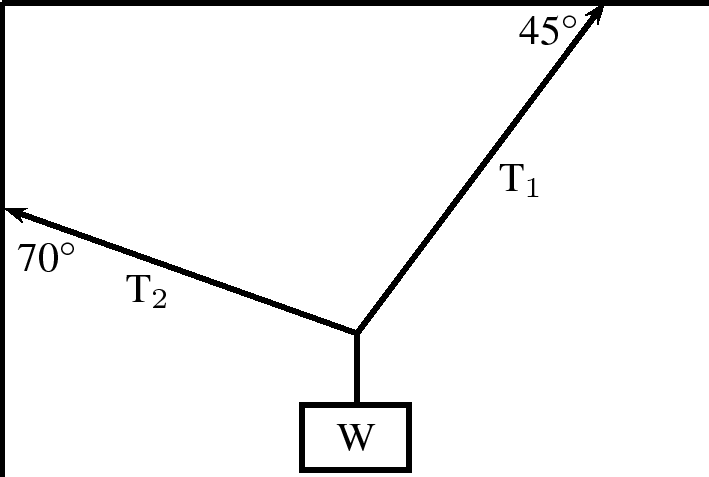
\includegraphics[width=5cm]{col11305.imgs/m38819_PG11C1_080.png} % m38819;PG11C1\_080.png;;;6.0;8.5;
      \vspace{2pt}
    \vspace{.1in}
    \end{center}
 \end{figure}               \label{m38819*uid136}\item In a map-work exercise, hikers are required to walk from a tree marked A on the map to another tree marked B which lies 2,0 km due East of A. The hikers then walk in a straight line to a waterfall in position C which has components measured from B of 1,0 km E and 4,0 km N.
\label{m38819*id198765}\begin{enumerate}[noitemsep, label=\textbf{\alph*}. ] 
            \label{m38819*uid137}\item Distinguish between quantities that are described as being \textsl{vector} and \textsl{scalar}.
\label{m38819*uid138}\item Draw a labeled displacement-vector diagram (not necessarily to scale) of the hikers' complete journey.
\label{m38819*uid139}\item What is the total distance walked by the hikers from their starting point at A to the waterfall C?
\label{m38819*uid140}\item What are the magnitude and bearing, to the nearest degree, of the displacement of the hikers from their starting point to the waterfall?
\end{enumerate}
                \label{m38819*uid141}\item An object $X$ is supported by two strings, $A$ and $B$, attached to the ceiling as shown in the sketch. Each of these strings can withstand a maximum force of 700~N. The weight of $X$ is increased gradually.
\label{m38819*id198883}\begin{enumerate}[noitemsep, label=\textbf{\alph*}. ] 
            \label{m38819*uid142}\item Draw a rough sketch of the triangle of forces, and use it to explain which string will break first.
\label{m38819*uid143}\item Determine the maximum weight of $X$ which can be supported.
\end{enumerate}
    \setcounter{subfigure}{0}
	\begin{figure}[H] % horizontal\label{m38819*id198922}
    \begin{center}
    \label{m38819*id198922!!!underscore!!!media}\label{m38819*id198922!!!underscore!!!printimage}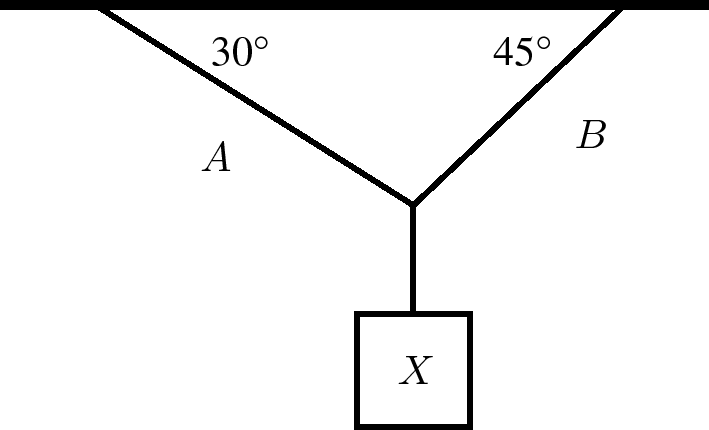
\includegraphics[width=5cm]{col11305.imgs/m38819_PG11C1_081.png} % m38819;PG11C1\_081.png;;;6.0;8.5;
      \vspace{2pt}
    \vspace{.1in}
    \end{center}
 \end{figure}               \label{m38819*uid144}\item A rope is tied at two points which are 70~cm apart from each other, on the same horizontal line. The total length of rope is 1~m, and the maximum tension it can withstand in any part is 1000~N. Find the largest mass ($m$), in kg, that can be carried at the midpoint of the rope, without breaking the rope. Include a vector diagram in your answer.
    \setcounter{subfigure}{0}
	\begin{figure}[H] % horizontal\label{m38819*id198958}
    \begin{center}
    \label{m38819*id198958!!!underscore!!!media}\label{m38819*id198958!!!underscore!!!printimage}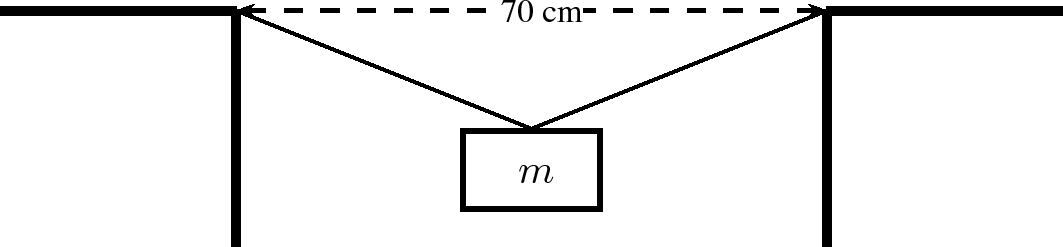
\includegraphics[width=300px]{col11305.imgs/m38819_PG11C1_082.png} % m38819;PG11C1\_082.png;;;6.0;8.5;
      \vspace{2pt}
    \vspace{.1in}
    \end{center}
 \end{figure}               \end{enumerate}
  \label{m38819**end}
  \label{59e414b70efc194a27a122db47d06ce6**end}
\par \raisebox{-5 pt}{
\includegraphics[width=0.5cm]{col11305.imgs/summary_www.png}} Find the answers with the shortcodes:
 \par \begin{tabular}[h]{cccccc}
 (1.) l25  &  (2.) l2N  &  (3.) l2R  &  (4.) l2n  &  (5.) l2E  &  (6.) l2m  &  (7.) l2y  &  (8.) l2V  &  (9.) l2p  & \end{tabular}
